\subsection{THz radiation source}
\label{subsec:rot:radiation-source}

A continuous wave Signal Generator Extension (SGX) Module (VDI - Virginia Diode, Inc. WR9.0-SGX) has been used to measure pure rotational transitions of molecular ions. The SGX covers the frequency range from 82.5 - 1100 GHz using different frequency doubler or tripler combinations. Table \ref{tab:vdi-multiplier} provides the configurations used in this thesis. The microwave signal generator (R\&S \textsuperscript{\textregistered} SMB100A up to 40 GHz) drives the SGX and is disciplined by an atomic clock (Stanford Research Systems - FS740), such that the intrinsic radiation linewidths are better than 1~kHz, and the relative frequency accuracy is specified to be better than $1\cdot 10^{-13}$. The WR9.0 SGX was placed directly in front of a 0.6 mm thick CVD diamond window (Diamond Materials GmbH) with a conical/diagonal horn antenna and directed into the trap region. Figure \ref{fig:power-curves} shows the power output measured using a high sensitivity thermal sensor (3A-P-THz Ophir photonics) for configuration WR9.0 and WR2.2 SGX.

\begin{threeparttable}[!htb]
    \centering
    \caption{WR9.0M-SGX configuration details at standard RF input mode. }
    \begin{tabular}{cccc}
        \hline\\
        Designation & Frequency [GHz] & Configuration & N\tnote{*} \\
        \\\hline\hline\\
        WR9.0 & 82.5-125 & WR9.0SGX & 9 \\
        WR4.3 & 170-250 & WR9.0SGX + WR4.3X2 & 18 \\
        WR2.2 & 340-500 & WR9.0SGX + WR4.3X2 + WR2.2X2 & 36 \\
        \\\hline\hline
    \end{tabular}
    \begin{tablenotes}
        \item[*] N indicates the multiplier for signal generator (R\&S \textsuperscript{\textregistered} SMB100A) frequencies.\\
    \end{tablenotes}
    \label{tab:vdi-multiplier}
\end{threeparttable}

\begin{figure}[!htb]
    \Subfigure[0.48]{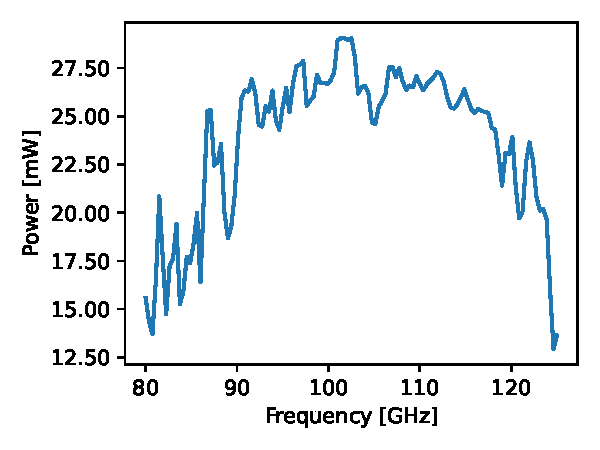
\includegraphics[width=1\textwidth]{figures/measurements/power-curves/WR9.0M.pdf}}{WR9.0}{\label{fig:power-curve:WR9.0}}
    \hfill
    \Subfigure[0.48]{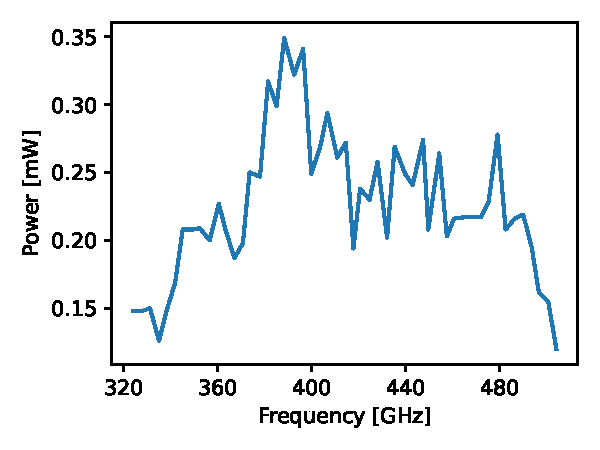
\includegraphics[width=1\textwidth]{figures/measurements/power-curves/WR2.2.pdf}}{WR2.2}{\label{fig:power-curve:WR2.2}}
    \hfill

    \caption{Power curves measured with Virginia Diodes, Inc.(VDI) WR9.0 Modular SGX Modules in (a) WR9.0 and (b) WR2.2 configuration as described in Table \ref{tab:vdi-multiplier}.}
    \label{fig:power-curves}
\end{figure}

\begin{figure}[!htb]
    \Subfigure[0.3]{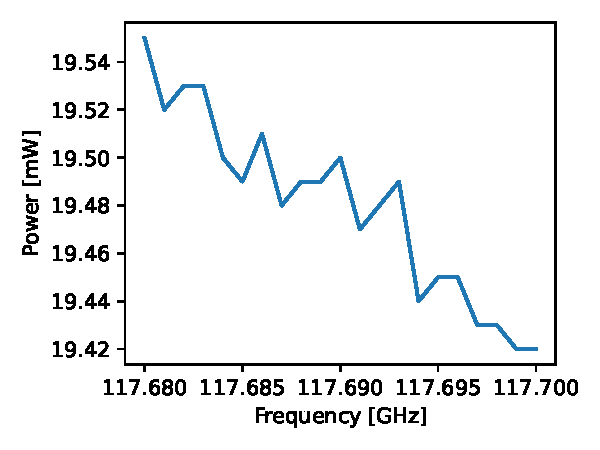
\includegraphics[width=1\textwidth]{figures/measurements/power-curves/WR9.0M_117GHz.pdf}}{}{}
    \hfill
    \Subfigure[0.3]{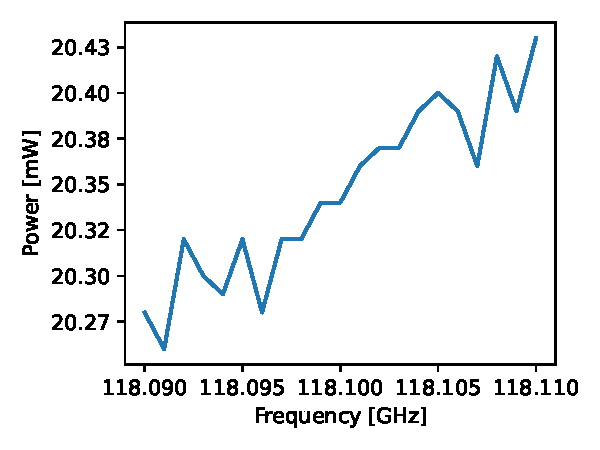
\includegraphics[width=1\textwidth]{figures/measurements/power-curves/WR9.0M_118GHz.pdf}}{}{}
    \hfill
    % \centering
    \Subfigure[0.3]{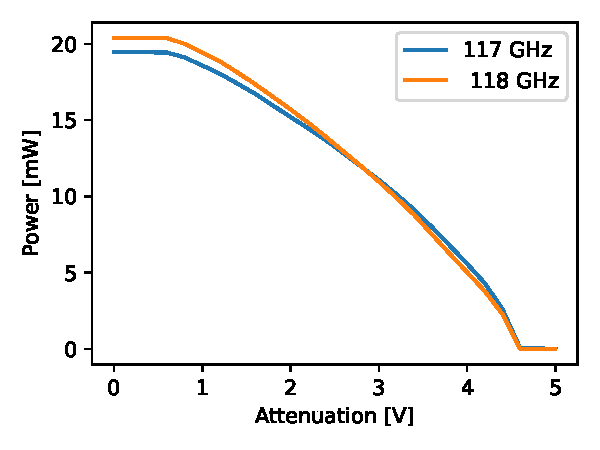
\includegraphics[width=1\textwidth]{figures/measurements/power-curves/WR9.0M_117GHz _att_WR9.0M_118GHz _att.pdf}}{}{\label{fig:power-attenuation-117-118}}
    \hfill
    \caption{Power curves measured with Virginia Diodes, Inc.(VDI) WR9.0 Modular SGX Modules in WR9.0 configuration, for the frequency ranges (a) $117.68-117.70$ GHz and (b) $118.09-118.11$ GHz. (c) shows the user-controlled attenuation power output for (a) and (b) as labelled 117 and 118 GHz, respectively. }
    \label{fig:power-attenuation}
\end{figure}

The maximum radiation output power can be regulated using \qt{User Controlled Attenuation (UCA)}. The UCA voltage reduces the SGX module's output power. Figure \ref{fig:power-attenuation} shows the WR9.0 SGX module output power as a function of UCA voltage from  $0-5$ V using a DC power supply (0 V = no attenuation, 5 V = full attenuation). The maximum output power reaching the trap centre region is discussed in the following section \ref{subsec:rot:power}.

\clearpage
